\chapter{Die speisenden Philosophen}
\label{speisende_philosophen}

%Referenzen wie in \ref{fazit}

%\begin{lstlisting}[style = Python, label = {mein_beispiel}, caption = {Das zeige ich euch}]
%print("Hallo das ist mein Programm")

%variable = true

%if variable:
%	print("Variable war true"!)

%\end{lstlisting}

%das ist ein test \parencite[S.4]{rechenberg2000}
\section{Vorstellung des Modells}
\label{vorstellung}
Das 1965 von Dijkstra formulierte Philosophenproblem lässt sich wie folgt darstellen: Fünf Philosophen sitzen an einem runden Tisch. Jeder der Philosophen hat einen Teller mit Spagetti vor sich und weil die Nudeln so schlupfrig sind, benötigt man zwei Gabeln um sie zu essen. So liegt zwischen jedem Teller eine Gabel. Zusammengefasst gibt es nun fünf Teller mit den Spagetti und fünf Gabeln. Nun hat jeder Philosoph eine bestimmte Reihenfolge wie sie diese Tätigkeiten ausführen. Diese ist fest und unaustauschbar. Erst denken die Philosophen und weil Denken so hungrig macht, essen sie danach und heben erst die linke und dann die rechte Gabel auf. Dies kann auch lange gut gehen. Aber was passiet wenn alle Philosophen gleichzeitig hungrig sind und gleichzeitig nach der, von ihnen aus, linken Gabel greifen? Wenn jeder Philosoph nach seiner linken Gabel greift, hat keiner seine rechte Gabel. Also werden die Philosophen verhungern.\parencite[vgl.][S.220]{tanenbaum2016} 


Nun werden die Philosophen durch Prozesse ersetzt und die Gabeln durch Betriebsmittel und es kristalisiert sich eine Verklemmung heraus denn alle vier Bedingungen sind erfüllt. \textit{Mutual exclusion}, da die Philosophen nicht zur selben Zeit mit der gleichen Gabel essen können. \textit{Hold and wait}, da die Philosophen immer zuerst an sich denken und die Gabel keinem anderen überlassen. \textit{No preemption}, die Philosophen sind gebildete Leute mit Manieren. Sie reißen einem anderem keine Gabel aus der Hand. Weil die Philosophen an einem runden Tisch sitzen und jeder auf die rechte Gabel wartet wird auch das \textit{Zirkuläre Warten} erfüllt.

\section{Darstellung des Problems}
\label{problem}
Um so ein Problem ausfindig zu machen, gibt es verschiedene Möglichkeiten so eine Verklemmung grafisch darzustellen. Um das Problem auflösen zu können, muss es erst sichtbar gemacht werden. Vorgestellt wird zuerst der Betriebsmittelbelegungsgraph. Bei diesem werden die Prozesse mit Kreis und die Betriebsmittel mit Quadrat dargestellt. Diese werden mit Knoten bezeichnet. Die Belegung und Anforderung auf Betriebsmittel wird mit Pfeilen, auch Kanten genannt, dargestellt. Kommt dabei der Pfeil von dem Betriebsmittel zu dem Prozess, so bedeutet das, dass der Prozess dieses schon im Besitz hat. Verläuft der Pfeil von Prozess zu Betriebsmittel so stellt der Prozess die Anforderung an das Betriebsmittel. Der Grundaufbau wird in Abbildung \ref{fig:normaler_betriebsmittelbelegungsgraph} gezeigt.

\begin{figure}[h]
\caption{Normaler Betriebsmittelbelegungsgraph}
\label{fig:normaler_betriebsmittelbelegungsgraph}
\centering
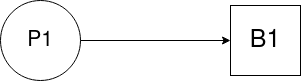
\includegraphics[width=.4\linewidth]{Belegungsgraph1.png}
\end{figure}

Bildet sich dabei eine zirkuläre Wartebeziehung so ist eine Verklemmung entstanden. 
P1 besitzt Betriebsmittel B3 und benötigt B1. P2 hat Betriebsmittel B1 im Besitz und stellt die Anforderung an B2, welches schon von P3 belegt ist. P3 belegt B3 und fordert B1 an. Damit schließt sich der Kreis und es entsteht eine Verklemmung, da die vorhandenen Prozesse in einer zirkulären Wartebeziehung stehen. Hier in Abbildung \ref{fig:verklemmter_betriebsmittelbelegungsgraph} wird ein verklemmter Betriebsmittelbelegungsgraph dargestellt.

\begin{figure}[H]
\caption{Bei diesem Beispiel liegt eine Verklemmung vor}
\label{fig:verklemmter_betriebsmittelbelegungsgraph}
\centering
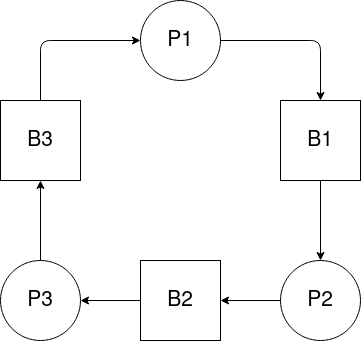
\includegraphics[width=.4\linewidth]{Belegungsgraph2.png}
\end{figure}

Eine andere Möglichkeit, eine Verklemmung darzustellen, ist das Prozess-Ablaufdiagramm. Bei letzterem werden die Prozesse auf der x- bzw. y-Achse dargestellt und deren Rechnung als Linie. Verläuft die Linie in y-Richtung, so rechnet P1, verläuft sie in x-Richtung, rechnet P2. Die in dem Diagramm dargestellten ``Ecken'' symbolisieren die Änderung des Rechenvorgangs von P1 auf P2. Auf jeden der Achsen sind außerdem die angeforderten Betriebsmittel gekennzeichnet. Das rote Feld kennzeichnet die Spanne wann ein Betriebsmittel belegt wird. In diesen Bereich können die Prozesse nicht hinein.
In Abbildung \ref{fig:normales_Ablaufdiagramm} wird ein normales Prozessablaufdiagramm ohne eine Verklemmung dargestellt.

\begin{figure}[H]
\caption{Möglicher Verlauf bei einem Prozessablaufdiagramm ohne Verklemmung}
\label{fig:normales_Ablaufdiagramm}
\centering
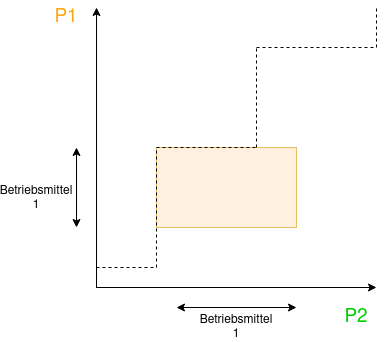
\includegraphics[width=.6\linewidth]{Prozess_Ablaufdiagramm.png}
\end{figure}

Nun wird ein zweites Betriebsmittel dazugenommen. Wie gewohnt rechnen die Prozesse jedoch kann bei dem Beispiel \ref{fig:verklemmtes_ablaufdiagramm} eine Verklemmung entstehen. Die Zahlen 1-3 stellen mögliche Abläufe der Prozesse dar. Bei Ablauf 1 und 3 entsteht keine Verklemmung denn diese laufen jeweils links(1) und unterhalb(3) der gekennzeichneten Bereiche. Sie könne ungehindert rechnen denn sie belegen die Betriebsmittel aber lassen sie anschließend wieder frei. Ablauf 3 jedoch gerät in den kritischen Abschnitt bis sich dann schließlich eine Verklemmung visuallisiert. Verläuft die Linie des 3. Ablaufs weiter vertikal, so entsteht eine Verklemmung denn Betriebsmittel 1 ist bereits von Prozess 1 belegt. Lässt er Prozess 1 weiterrechnen so entsteht eine Verklemmung, denn Betriebsmittel 2 ist bereits von Prozess 2 schoon in Beschlag genommen. Zusammengefasst, betritt die Linie 3 den roten Bereich so ist eine Verklemmung unvermeidbar.
Eine Verklemmung ist bei einem solchen Diagramm nur möglich, wenn sich die Bereiche (in dieser Abbildung orange und grün gekennzeichnet) der Betriebsmittel überschneiden.

\begin{figure}[H]
\caption{Beispiel eines Prozessablaufdiagrammes mit Verklemmung}
\label{fig:verklemmtes_ablaufdiagramm}
\centering
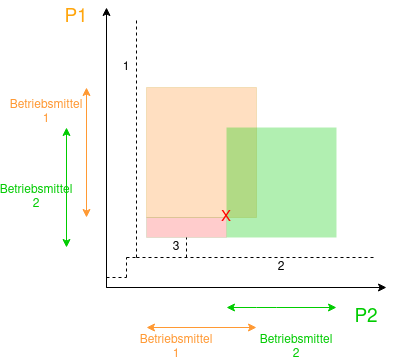
\includegraphics[width=.6\linewidth]{prozessablaufdiagramm2.png}
\end{figure}

\section{Lösungsansätze}
\label{lösung}

